% bei Standalone in documentclass noch:
% \RequirePackage{luatex85}

\documentclass[captions=tableheading, titlepage= firstiscover, parskip = half , bibliography=totoc]{scrartcl}
%paper = a5 fÃŒr andere optinen
% titlepage= firstiscover
% bibliography=totoc fÃŒr bibdateien
% parskip=half  VerÀnderung um AbsÀtze zu verbessern

\usepackage{scrhack} % nach \documentclass
\usepackage[aux]{rerunfilecheck}
\usepackage{polyglossia}
\usepackage[style=numeric, backend=biber]{biblatex} % mit [style = alphabetic oder numeric] nach polyglossia
\addbibresource{lit.bib}
\setmainlanguage{german}

\usepackage[autostyle]{csquotes}
\usepackage{amsmath} % unverzichtbare Mathe-Befehle
\usepackage{amssymb} % viele Mathe-Symbole
\usepackage{mathtools} % Erweiterungen fÃŒr amsmath
\usepackage{fontspec} % nach amssymb
% muss ins document: \usefonttheme{professionalfonts} % fÌr Beamer PrÀsentationen
\usepackage{longtable}
\usepackage{dsfont}
\usepackage[
math-style=ISO,    % \
bold-style=ISO,    % |
sans-style=italic, % | ISO-Standard folgen
nabla=upright,     % |
partial=upright,   % /
]{unicode-math} % "Does exactly what it says on the tin."
\setmathfont{Latin Modern Math}
% \setmathfont{Tex Gyre Pagella Math} % alternativ

\usepackage[
% die folgenden 3 nur einschalten bei documenten
locale=DE,
separate-uncertainty=true, % Immer Fehler mit ±
per-mode=symbol-or-fraction, % m/s im Text, sonst \frac
]{siunitx}

% alternativ:
% per-mode=reciprocal, % m s^{-1}
% output-decimal-marker=., % . statt , fÃŒr Dezimalzahlen

\usepackage[
version=4,
math-greek=default,
text-greek=default,
]{mhchem}

\usepackage[section, below]{placeins}
\usepackage{caption} % Captions schöner machen
\usepackage{graphicx}
\usepackage{grffile}
\usepackage{subcaption}

% \usepackage{showframe} Wenn man die Ramen sehen will

\usepackage{float}
\floatplacement{figure}{htbp}
\floatplacement{table}{htbp}

\usepackage{mathtools}

\usepackage{booktabs}

 \usepackage{microtype}
 \usepackage{xfrac}

 \usepackage{expl3}
 \usepackage{xparse}

 % \ExplSyntaxOn
 % \NewDocumentComman \I {}  %Befehl\I definieren, keine Argumente
 % {
 %    \symup{i}              %Ergebnis von \I
 % }
 % \ExplSyntaxOff

 \usepackage{pdflscape}
 \usepackage{mleftright}

 % Mit dem mathtools-Befehl \DeclarePairedDelimiter können Befehle erzeugen werden,
 % die Symbole um AusdrÃŒcke setzen.
 % \DeclarePairedDelimiter{\abs}{\lvert}{\rvert}
 % \DeclarePairedDelimiter{\norm}{\lVert}{\rVert}
 % in Mathe:
 %\abs{x} \abs*{\frac{1}{x}}
 %\norm{\symbf{y}}

 % FÃŒr Physik IV und Quantenmechanik
 \DeclarePairedDelimiter{\bra}{\langle}{\rvert}
 \DeclarePairedDelimiter{\ket}{\lvert}{\rangle}
 % <name> <#arguments> <left> <right> <body>
 \DeclarePairedDelimiterX{\braket}[2]{\langle}{\rangle}{
 #1 \delimsize| #2
 }

\setlength{\delimitershortfall}{-1sp}

 \usepackage{tikz}
 \usepackage{tikz-feynman}

 \usepackage{csvsimple}
 % Tabellen mit \csvautobooktabular{"file"}
 % muss in table umgebung gesetzt werden


% \multicolumn{#Spalten}{Ausrichtung}{Inhalt}

\usepackage{hyperref}
\usepackage{bookmark}
\usepackage[shortcuts]{extdash} %nach hyperref, bookmark

\newcommand{\ua}[1]{_\symup{#1}}
\newcommand{\su}[1]{\symup{#1}}

\begin{document}
\section{Zielsetzung}
In diesem Versuch sollen für die Rubidium-Isotope $^{85}\su{Rb}$ und $^{87}\su{Rb}$ die Landé-Faktoren und die
daraus folgenden Spins der Elektronenhülle und des Kernspins mittels des optischen Pumpens bestimmt werden.
\section{Theorie}
Die Elektronenhüllen eines isolierten Atoms besitzen diskrete Energieniveaus. Die innersten Schalen sind nach dem Paulischen Ausschließungsprinzip
vollständig mit Elektronen besetzt. Bei äußeren Energieniveaus hingegen kommt es
zur temperaturabhängigen Besetzung. Diese wird durch die Boltzmannsche Gleichung
\begin{align}
    \frac{N_{2}}{N_{1}} = \frac{g_{2}}{g_{1}}\frac{\exp(-W_{2}/\su{kT})}{\exp(-W_{1}/\su{kT})}
    \label{eqn:boltzmann}
\end{align}
mit den Zuständen $N_1$, $N_2$ und den Energien $W_1$, $W_2$
beschreiben. Die statistischen Gewichte $g_{\text{i}}$ geben hierbei die Anzahl der zu der Energie
$W_{\text{i}}$ gehörigen Zustände an.
Durch das optische Pumpen ist es möglich, die in \ref{eqn:boltzmann} gegebene Verteilung
zu verändern und schließlich sogar Inversion der Besetzungszustände mit $N_2 > N_1$ zu erzeugen.
Diese Inversion kann dann zur Induzierung von Strahlungsübergängen verwendet werden.
Die Energiedifferenz
\begin{align*}
    h\nu = W_{2}-W_{1}
\end{align*}
kann für kleine Energien mithilfe der Hyperfeinstrukturaufspaltung und
Zeeman-Aufspaltung präzise bestimmt werden.

\subsection{Zeeman-Effekt}
In der ersten Näherung wird davon ausgegangen, dass die beiden Rubidium-Isotope einen verschwindenen
Kernspin besitzen. Der Gesamtdrehimpuls der Elektronenhülle $\vec{J}$ koppelt an ein
magnetisches Moment $\vec{\mu_{\su{J}}}$, was durch
\begin{align*}
    \vec{\mu_{\su{j}}} &= -g_{\su{j}} \mu_{\su{B}} \vec{J} \\
    |\vec{\mu_{\su{j}}}| &= g_{\su{j}} \mu_{\su{B}} \sqrt{J(J+1)}
\end{align*}
beschrieben wird. Dabei ist $\mu_{\su{B}}$ das Bohrsche Magneton, $g_{\su{j}}$ der Landé-Faktor, welcher
die Zusammensetzung des magnetischen Moments aus Bahndrehimpuls $\vec{L}$ und Spin $\vec{S}$ berücksichtigt.
Es folgt für das Gesamtmoment
\begin{align*}
    \vec{\mu_{\su{J}}} = \vec{\mu_{\su{L}}} + \vec{\mu_{\su{S}}}.
\end{align*}
Beim Anlegen eines Magnetfeldes B kommt es zur Energieaniveauaufspaltung in $2J+1$ Unterniveaus
\begin{align*}
    U_{\su{magn}} = M_{\su{J}} g_{\su{J}} \mu_{\su{B}} \su{B}.
\end{align*}
Diese Niveaufspaltung wird als Zeeman-Effekt bezeichnet.

\subsection{Hyperfeinstrukturaufspaltung}
Da die Rubidium-Isotope keinen verschwindenden Kernspin besitzen, muss die Hyperfeinstruktur der
einzelnen Energieniveaus und der daraus folgende Einfluss auf die Zeeman-Aufspaltung berücksichtigt werden.
Der Kernspin $\vec{I}$ koppelt dann mit dem Gesamtdrehimpuls des Elektronenhülle $\vec{J}$ zum Gesamtdrehimpuls
des Atoms
\begin{align*}
    \vec{F} = \vec{J} + \vec{I}.
\end{align*}
Die Quantenzahl $F$ kann die Werte von $I+J$ bis $|I-J|$ annehmen und spaltet folglich in die Hyperfeinstrukturterme für den ersten Fall mit $J<I$: $2J+1$, und für den zweiten Fall mit
$J>I$: $2I+1$.
Durch das Anlegen eines äußeren Magnetfeldes kommt es zur weiteren Aufspaltung der Hyperfeinstrukturterme
in $2F+1$-Zeeman-Niveaus. Die Energiedifferenz zweier benachbarter Niveaus wird bestimmt durch
\begin{align*}
    U_{\symup{HF}} = g_{\symup{F}} \mu_{\symup{B}} B.
\end{align*}
Der Landé-Faktor $g_{\symup{F}}$ folgt aus der vektoriellen Betrachtung
\begin{align*}
    g_{\su{F}} \approx g_{\su{J}} \frac{F(F+1)+J(J+1)-I(I+1)}{2F(F+1)}.
\end{align*}
Dies ist für ein Alkali Atom mit $J=\frac{1}{2}$ und $I=\frac{3}{2}$ beispielhaft in Abbildung \ref{fig:alkali}
dargestellt.
\begin{figure}
    \centering
    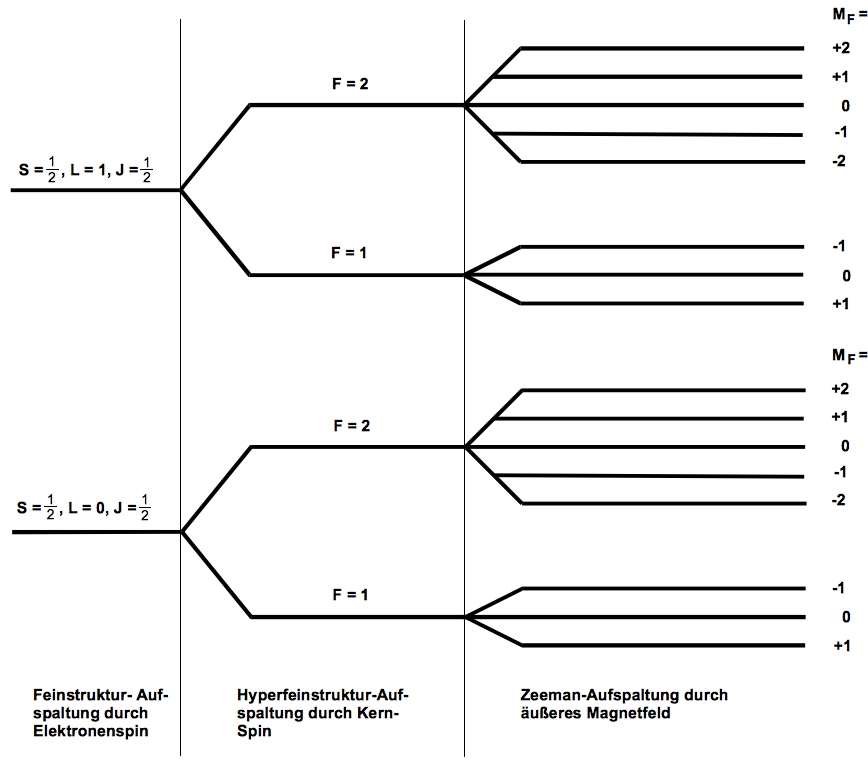
\includegraphics[scale = 0.54]{pictures/alkali.png}
    \caption{Hyperfeinstruktur- und Zeeman-Aufspaltung für einen $L=0$- und $L=1$-Zustand.\cite{1}}
    \label{fig:alkali}
\end{figure}

\newpage
\subsection{Optisches Pumpen}
Der Übergang in ein anderes Niveau kann nur unter Berücksichtigung der Auswahlregeln
$\Delta M_{\su{J}} = 0, \pm1$ erfolgen. Diese Übergänge unterschieden sich in ihrer Energie
und Polarisation.
Der $\sigma^{+}$-Übergang mit $\Delta M_{\text{J}} = +1$ kann nur mit rechszirkular-polarisierten Licht hervorgerufen werden,
wohingegen der $\sigma^{-}$-Übergang mit $\Delta M_{\text{J}} = -1$ mit linkszirkular-polarisierten.
Diese beiden Übergänge emittieren zirkular-polarisiertes Licht in Magnetfeldrichtung.
Der $\pi$-Übergang mit $\Delta M_{\text{J}} = 0$ emittiert parallel zum Magnetfeld linear polarisiertes
Licht. \newline
Die Zeeman-Aufspaltun mit den unterschiedlichen Übergängen und unter Vernachlässigung des Kernspins ist in Abbildung \ref{fig:übergänge}
für eine hypothetisches Alkali-Atom dargestellt.
\begin{figure}
    \centering
    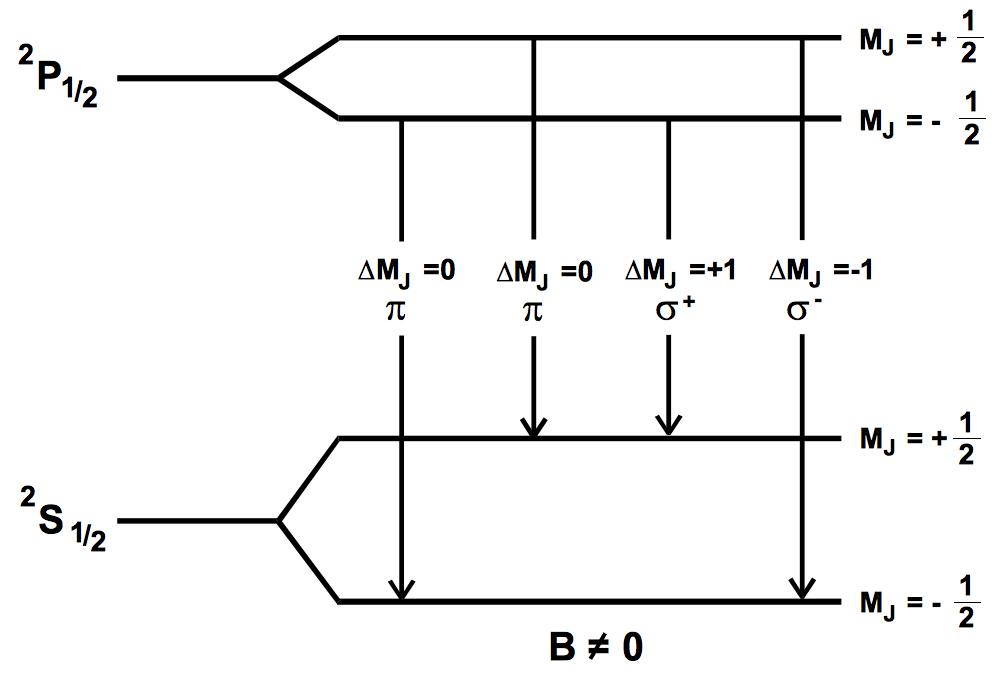
\includegraphics[scale = 0.35]{pictures/übergänge.png}
    \caption{Zeeman-Aufspaltung des Alkali-Atoms unter Vernachlässigung des Kernspins.\cite{1}}
    \label{fig:übergänge}
\end{figure}

Durch das Einstrahlen von rechtszirkular-polarisierten $D_{\su{1}}$-Licht und das Anlegen eines Magnetfeldes
kann ein aus hypothetisches Alkali-Atomen, welche sich alles im thermischen Gleichgewicht befinden, bestehender Dampf
in einen angeregten Zustand übergehen.
Die möglichen Übergänge für diese Alkali-Atome sind in Abbildung \ref{fig:übergängerechts} zu sehen.
\begin{figure}
    \centering
    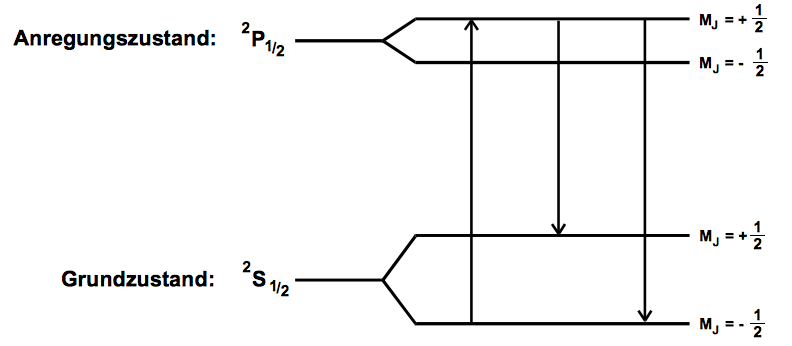
\includegraphics[scale = 0.4]{pictures/übergängerechts.png}
    \caption{Übergangsmöglichkeiten für dieses Beispiel.\cite{1}}
    \label{fig:übergängerechts}
\end{figure}
\newline
Durch das eingestrahlte rechtszirkular-polarisierte Licht werden jediglich $\Delta M_{\su{J}} = +1$-Übergänge angeregt, weshalb
nur der Übergang von $^{2}S_{\su{\frac{1}{2}}}$ $M_{\su{J}}=-\su{\frac{1}{2}}$ zu $^{2}P_{\su{\frac{1}{2}}}$ $M_{\su{J}}=+\su{\frac{1}{2}}$
möglich ist. Die spontane Emission, bei der ein Photon aus einem angeregten Atom emittiert wird, führt zum Übergang
zurück in den Grundzustand. Der Grundzustand besteht dabei aus den Niveaus $^{2}S_{\su{\frac{1}{2}}}$ $M_{\su{J}}=+\su{\frac{1}{2}}$ und
$^{2}S_{\su{\frac{1}{2}}}$ $M_{\su{J}}=-\su{\frac{1}{2}}$. Da allerdings der $\sigma^{+}$-Übergang bei $^{2}S_{\su{\frac{1}{2}}}$ $M_{\su{J}}=+\su{\frac{1}{2}}$
nicht in die P-Niveaus möglich ist, reichern sich in dem anderen Zustand die Elektronen an, währenddessen der energetisch niedrigerere Zustand zunehmend weniger besetzt und
irgendwann sogar leer gepumpt wird.

Die Inversion der Besetzung kann mittels einer Intensitätsmessung nach Durchtritt des Lichts durch die Dampfzelle
mithilfe eines Detektors nachgewiesen werden. Durch die Entleerung des $M_{\su{J}}= -\frac{1}{2}$-Zustandes
wird das einfallende Licht immer weniger absorbiert.
Die Transparenz der Dampfzelle nimmt dadurch zu und läuft asymptotisch gegen den Wert 1, wenn es möglich ist diesen Zustand
leer zu pumpen. Dies ist in Abbildung \ref{fig:asymptotisch} dargestellt.
\begin{figure}
    \centering
    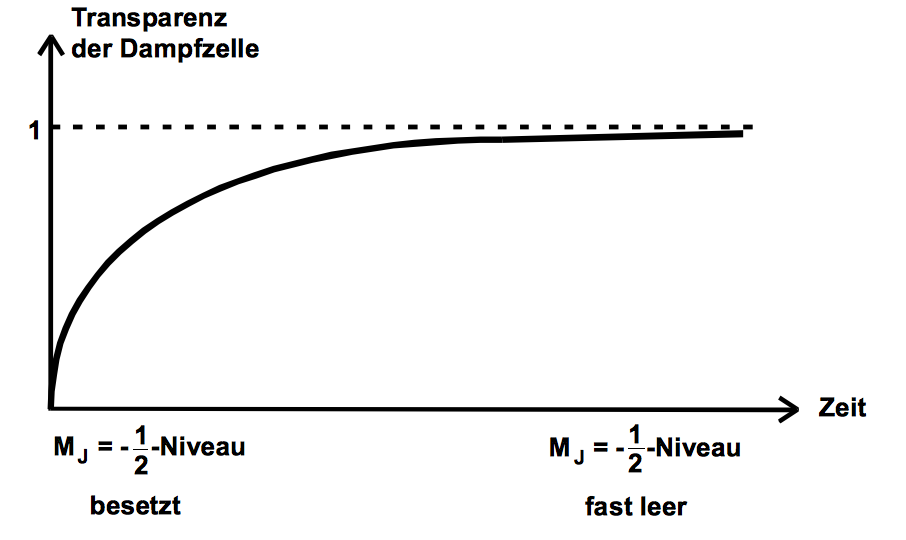
\includegraphics[scale = 0.6]{pictures/asymptotisch.png}
    \caption{Entwicklung der Transparenz unter Einstrahlung des rechtszirkular-polarisierten Lichts.\cite{1}}
    \label{fig:asymptotisch}
\end{figure}

\noindent Neben der zuvor erwähnten spontanen Emission gibt es noch die induzierte Emission von Lichtquanten bei der
die Emission nur durch ein eingestrahltes Photon stattfindet, welches genau die Energie
des Überganges haben muss. Die beiden Photonen stimmen dann in Energie, Ausbreitungsrichtung und Polarisation überein.
Diese beiden Emissionsformen können parallel geschehen. Im Energiebereich der Zeeman-Aufspaltung
kann die spontane Emission allerdings vernachlässigt werden und es findet hauptsächlich induzierte
Emission statt. In Abbildung \ref{fig:emission} sind die unterschiedlichen Emissionsformen skizziert.
\begin{figure}
    \centering
    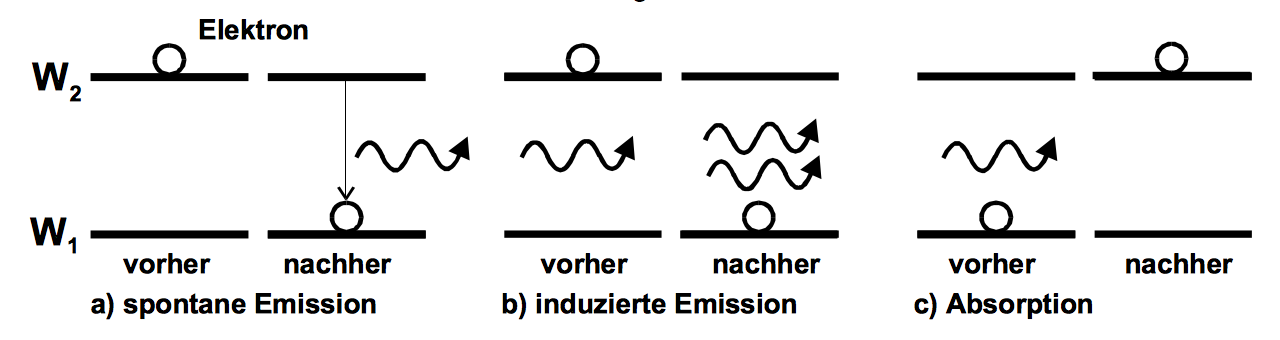
\includegraphics[scale = 0.5]{pictures/emission.png}
    \caption{Übergangsmöglichkeiter einer Elektrons zwischen zwei Energieniveaus.\cite{1}}
    \label{fig:emission}
\end{figure}

\noindent Durch ein frequenzvariables Hochfrequenzfeld kann die induzierte Emission hervorgerufen werden.
Über den Zusammenhang
\begin{align*}
    h\nu = g_{\su{J}} \mu_{\su{B}} B_{\su{m}} \Delta M_{\su{J}}
\end{align*}
kann der Wert für das Magnetfeld
\begin{align*}
    B_{\su{m}} = \frac{4\pi m_{\su{0}}} {e_{\su{0}} g_{\su{J}}} \nu
\end{align*}
bestimmt werden ab dem die induzierte Emission einsetzt. Dies hat zur Folge, dass das
$^{2}S_{\su{\frac{1}{2}}}$ $M_{\su{J}}=+\su{\frac{1}{2}}$ leergepumpt wird, das
$^{2}S_{\su{\frac{1}{2}}}$ $M_{\su{J}}=-\su{\frac{1}{2}}$ ausgefüllt wird und somit
das in die Dampfzelle eingestrahlte Licht wieder absorbiert werden kann.
Im Resonanzfall nimmt die Transparenz der Dampfzelle ab, wie in Abbildung \ref{fig:resonanz}
dargestellt ist.
\begin{figure}
    \centering
    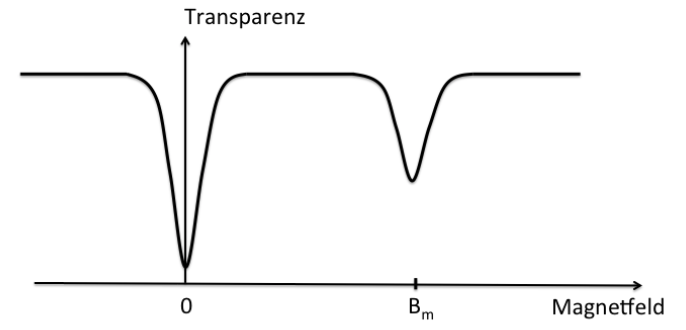
\includegraphics[scale = 0.6]{pictures/resonanz.png}
    \caption{Transparenz der Dampfzelle für rechtszirkular-polarisiertes Licht.\cite{1}}
    \label{fig:resonanz}
\end{figure}

\newpage
\subsection{Quadratischer Zeeman-Effekt}
Für größere Magnetfelder können Terme höherer Ordnung nicht vernachlässigt werden.
Durch Lösen der Schrödingergleichung
\begin{align*}
    H \Psi = U \Psi
\end{align*}
mit dem Hamilton-Operator, der sowohl die Spin-Bahn-Wechselwirkung, als auch die Wechselwirkungen
der magnetischen Momente beinhaltet, folgt für die Übergangsenergie
\begin{align*}
     U_{\su{HF}} = g_{\su{F}} \mu{_\su{B}} \su{B} + g_{\su{F}}^2 \mu{_\su{B}}^2 \su{B}^2 \frac{(1-2M_{\su{F}})}{\symup\Delta E_{\su{HF}}} -\,...,
\end{align*}
mit der Energiedifferenz $\Delta E_{\symup{HF}}$ zwischen den Niveaus $F$ und $F+1$. Die Übergangsenergie ist in dem
zusätzlichen Term proportional zu $B^2$. Die Zeeman-Energie ist abhänig von der Quantenzahl $M_{\symup{F}}$.\\
Dies wird als quadratischer Zeeman-Effekt bezeichnet.

\subsection{Transiente Effekte}
Bei der Betrachtung von gepumpten Systemen bei denen die Hochfrequenz innerhalb kürzester Zeit ein- und wieder ausgeschaltet wird,
ist die Resonanzfreuqenz gegeben durch
\begin{align*}
    \omega_{\symup{0}} = 2 \pi \nu_{\symup{0}} = g_{\symup{f}} \frac{\nu_{\su{0}}}{h} B_{\su{0}},
\end{align*}
wobei die Larmor-Frequenz durch $\omega_{\su{0}} = \gamma B_{\su{0}}$ mit dem gyromagnetischen Verhältnis
$\gamma = g_{\su{f}} \frac{\mu_{\su{0}}}{h}$ beschrieben wird.
Für den Resonanzfall ergibt sich $B_{\text{RF}} = B_{\text{eff}}$.
\newline
In diesem Fall folgt die Relation
\begin{align*}
    \frac{T_{\su{87}}}{T_{\su{85}}} = \frac{\gamma_{\su{85}}}{\gamma_{\su{87}}}
\end{align*}
für die beiden Rubidium-Isotope.

\newpage
\section{Aufbau}
In Abbildung \ref{fig:aufbau} ist der verwendete Versuchsaufbau dargestellt.
\begin{figure}
    \centering
    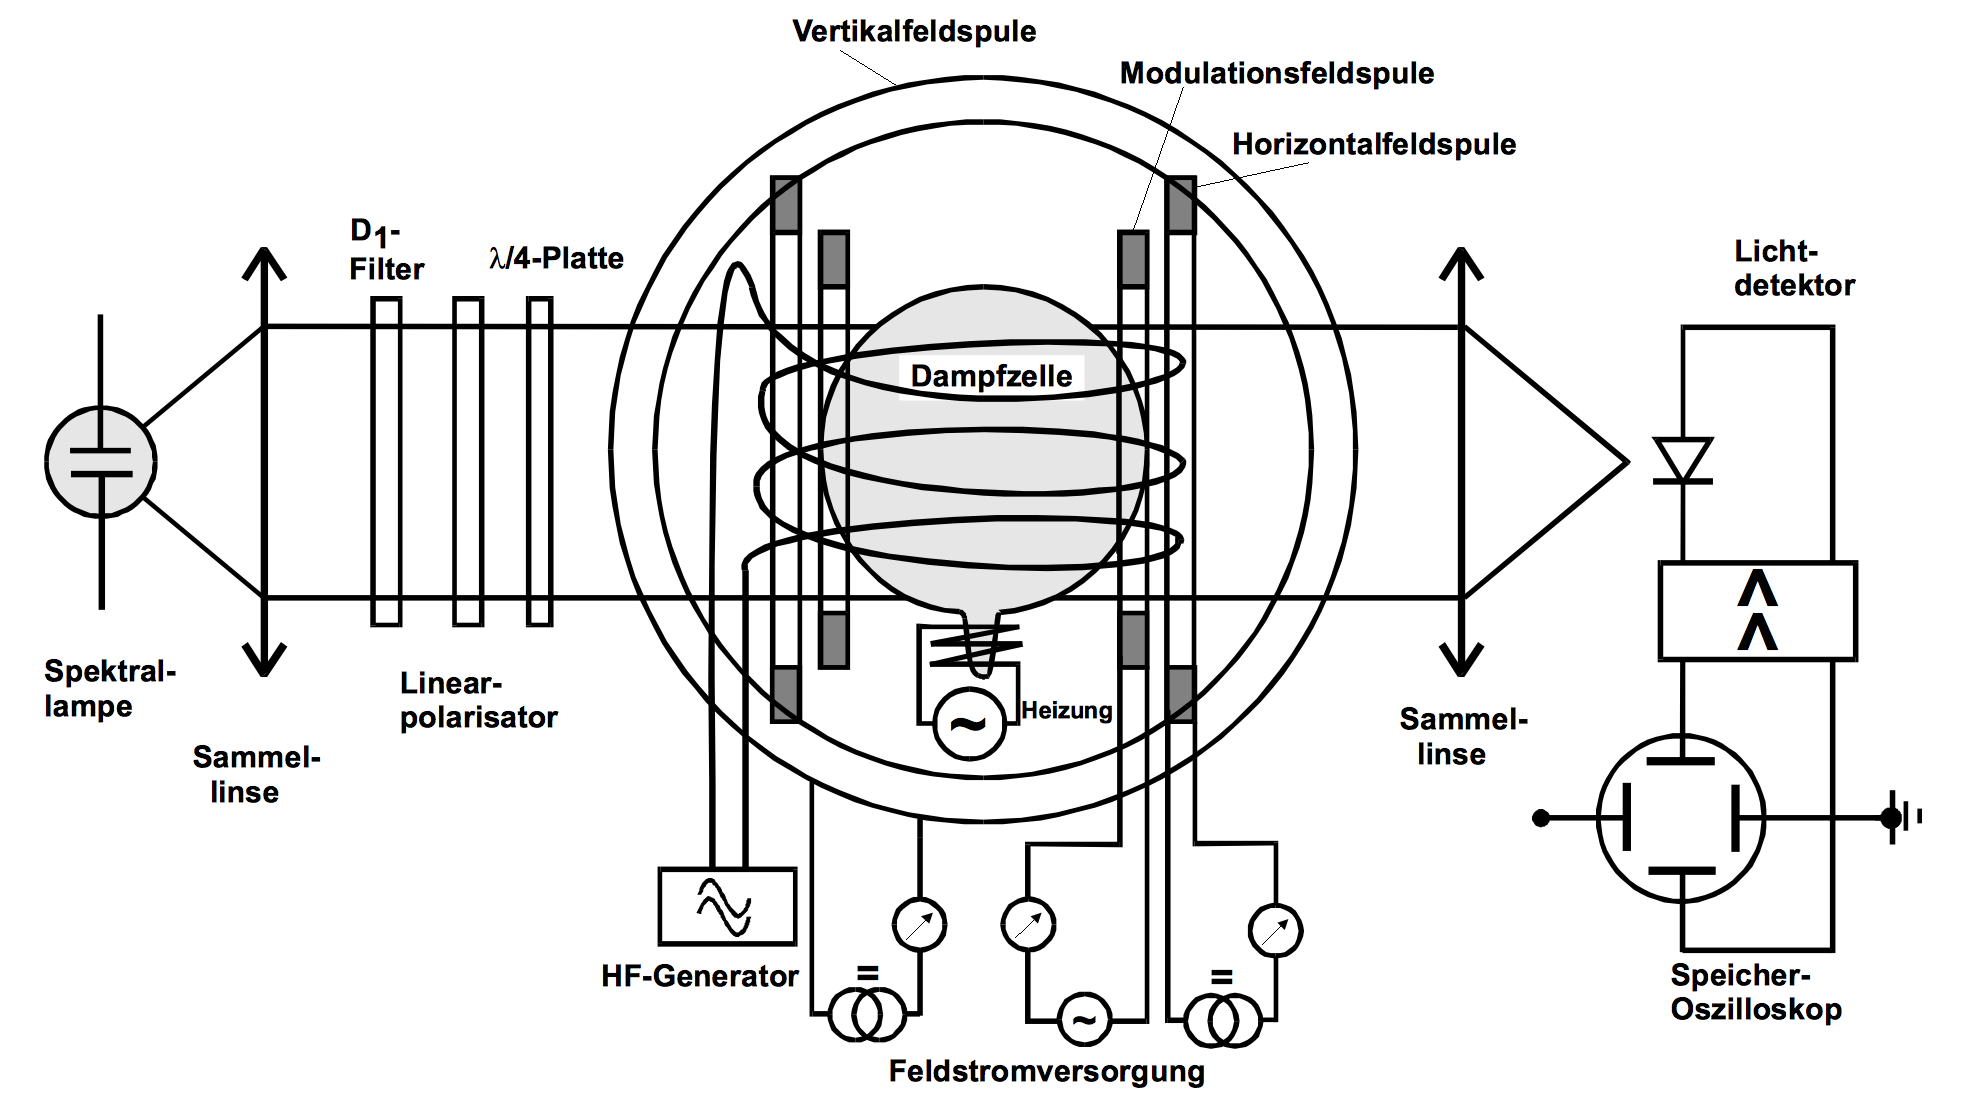
\includegraphics[scale = 0.4]{pictures/aufbau.png}
    \caption{Darstellung des Versuchsaufbaus.\cite{1}}
    \label{fig:aufbau}
\end{figure}
\newline
Das aus der Spektrallampe austretende Licht wird mithilfe einer Sammellinse kollimiert und durch einen $\text{D}_{\su{1}}$-Filter,
welcher nur die zu untersuchende $\text{D}_{\su{1}}$-Linie der Rubidium-Isotope durchlässt, gefiltert.
Der Linearpolarisationsfilter und die $\frac{\lambda}{4}$-Platte im Anschluss sorgen dafür, dass das
aus dem zuvor austretenden Licht zirkular-polarisiertes Licht erzeugt wird. Dieses trifft auf die Dampfzelle, in der
sich die beiden Rubidium-Isotope befinden. Durch das Beheizen der Dampfzelle wird ein optimaler Rubidium-Dampfdruck
eingestellt. Um das durchgetretene Licht auf ein Si-Photoelement zu fokussieren, wird
eine weitere Sammellinse verwendet. An das Photoelement angeschlossen sind ein Linearverstärker
und ein Oszilloskop mit dem sich Intensitätsänderungen des Lichtes darstellen lassen.

\noindent Um die Dampfzelle herum sind drei Helmholtz-Spulenpaare aufgestellt. Dabei gleicht die eine das wirkende
Erdmagnetfeld aus, wobei die anderen beiden für die Erzeugung der Zeeman-Aufspaltung der
Energieniveaus benötigt werden. Für die Erzeugung der horizontalen Feldern ist eine Sweep-Spule auf ein Horizontalfeld-Spule
gewickelt. \newline
Das durch eine weitere Spule entstandendene RF-Feld dient dazu, dass die Energieübergange abhängig von
der Horizontalfeldstärke sind.

\section{Durchführung}
Durch schrittweises Einstellen und Platzieren der beiden Sammellinsen wird die auf den Lichtdetektor
treffende Intensität versucht zu maximieren. Nach dem Einsetzen zusätzlicher optischer Elemente wird
der Versuchausaufbau durch eine Decke abgedunkelt.

Die Kompensation des Erdmagnetfelds mithilfe der Vertikal-Spule und der Drehung der Versuchsapparatur in der
horizontalen Ebene führt dazu, dass der auf dem Oszilloskop zu sehende Peak der Sweep-Spule und des Potentiometers
schmaler wird.

Für die Bestimmung der Resonanzstelle wird die Frequenz der RF-Spule in einem Bereich von 100\,kHz bis
1\,MHz schrittweise um 100\,kHz erhöht. Eine Sinusspannung wird zusätzlich angelegt.
Damit die Resonanzstellen der unterschiedlichen Frequenzen auf dem Oszilloskop zu sehen sind, wird
das Feld der Horizontalspule dementsprechend erhöht.
Ab einer Frequenz von ungefähr 200\,kHz muss ein weiteres horizontales Feld angelegt werden. Dies führt dazu,
dass der Bereich des Sweep-Feldes auf die einzelnen Resonanzen verschoben werden kann.

Nachdem die Ausgangsfrequenz von 100\,kHz und das Magnetfeld wieder auf die erste Resonanzstelle eingestellt ist,
wird eine Rechteckspannung von $0-5$\,V und mit einer Frequenz von 5\,Hz eingespeist. Dieses Signal
wird zusammen mit dem Signal des Si-Photoelements über den YT-Modus sichtbar gemacht.
Anhand der Aufnahmen des Oszilloskops kann über die Flanken der RF-Modulation
die Periode in Abhänigkeit der Amplitude bestimmt werden. Dafür wird die Amplitude im Bereich von $0,5$\,V bis 10\,V
in 1\,V Schritten verändert.
\end{document}
